%%%%%%%%%%%%%%%%%%%%%%% file template.tex %%%%%%%%%%%%%%%%%%%%%%%%%
%
% This is a general template file for the LaTeX package SVJour3
% for Springer journals.          Springer Heidelberg 2010/09/16
%
% Copy it to a new file with a new name and use it as the basis
% for your article. Delete % signs as needed.
%
% This template includes a few options for different layouts and
% content for various journals. Please consult a previous issue of
% your journal as needed.
%
%%%%%%%%%%%%%%%%%%%%%%%%%%%%%%%%%%%%%%%%%%%%%%%%%%%%%%%%%%%%%%%%%%%
%
%\documentclass{svjour3}                     % onecolumn (standard format)
%\documentclass[smallcondensed]{svjour3}     % onecolumn (ditto)
\documentclass[smallextended]{svjour3}       % onecolumn (second format)
%\documentclass[twocolumn]{svjour3}          % twocolumn
%
\smartqed  % flush right qed marks, e.g. at end of proof
%
\usepackage{graphicx}
\usepackage{amssymb}
\usepackage{amsmath}

\usepackage{hyperref}
\usepackage{cite}

%\usepackage[utf8x]{inputenc}
%\usepackage[english,russian]{babel}

%\usepackage{xcolor}

%\usepackage{academicons}
%\RequirePackage[colorlinks,citecolor=blue,urlcolor=blue]{hyperref}
%
% \usepackage{mathptmx}      % use Times fonts if available on your TeX system
%
% insert here the call for the packages your document requires
%\usepackage{latexsym}
% etc.
%
% please place your own definitions here and don't use \def but
% \newcommand{}{}
%
% Insert the name of "your journal" with
\journalname{Optimization Letters}
%
\begin{document}

\title{Computationally Efficient Approach for Solving Lexicographic Multicriteria Optimization Problems\thanks{The work was supported by the Ministry of Science and Higher Education of the Russian Federation, agreement No 075-15-2020-808. %``Novel efficient methods and software tools for time-consuming decision making problems using supercomputers of superior performance''.
}
}

\titlerunning{Efficient Approach for Solving Multicriteria Optimization Problems}        % if too long for running head

\author{Victor Gergel %\href{https://orcid.org/0000-0002-4013-2329}{
\includegraphics{ORCID.png}}
%\orcidID{0000-0002-4013-2329} 
\and
Evgeniy Kozinov
%\orcidID{0000-0001-6776-0096} 
\and
Konstantin Barkalov
%\orcidID{0000-0001-5273-2471}
}

%\authorrunning{Short form of author list} % if too long for running head

\institute{               
Victor Gergel \at
%\at Lobachevsky State University of Nizhni Novgorod, Nizhni Novgorod, Russia \\
\email{gergel@unn.ru} 
\and
Evgeniy Kozinov \at
%\at Lobachevsky State University of Nizhni Novgorod, Nizhni Novgorod, Russia \\
\email{evgeny.kozinov@itmm.unn.ru} 
\and
Konstantin Barkalov \at
%\at Lobachevsky State University of Nizhni Novgorod, Nizhni Novgorod, Russia \\
\email{konstantin.barkalov@itmm.unn.ru} \\
\at Mathematical Center, Lobachevsky State University of Nizhni Novgorod, Gagarin ave., 23, Nizhni Novgorod, Russia 
}

\date{Received: date / Accepted: date}
% The correct dates will be entered by the editor

\maketitle

\begin{abstract}
In this paper, we propose a computationally efficient approach for solving complex multicriteria lexicographic optimization problems, which can be complicated by the multiextremal nature of the efficiency criteria and extensive volume of computations required to calculate the criteria values. The formulation of problems is assumed to be the subject to change as well, which, in turn, may require solving dynamically defined sets of multicriteria optimization problems. The proposed approach is based on reducing multidimensional problems to one-dimensional global optimization problems, utilizing efficient global search algorithms, and reusing the search information obtained in the process of calculations. The results of numerical experiments confirm that the proposed approach demonstrates high computational efficiency of solving multicriteria global optimization problems.
\keywords{Multicriteria optimization \and Lexicographic ordering \and Global optimization \and Dimensional reduction \and Search information \and Computational complexity}
\end{abstract}

\section{Introduction}
\label{sec:1}

Multicriteria optimization (MCO) problems are among the most general statements used to address decision-making problems. These statements are commonly used in various applications. Multicriteria optimization is a dynamic area of scientific research. So far, researchers proposed a large number of efficient methods of multicriteria optimization and found solutions to many practical problems (see, e.g., monographs \cite{c1,c2,c3,c4,c5} and reviews \cite{c6,c7,c8,c9}).

A key aspect of MCO problems is the absence, in most cases, of a single decision, which would best satisfy all the efficiency criteria, since these criteria can be contradictory. As a result, solving MCO problems usually requires finding several compromise decisions (efficient and non-dominated) that cannot be improved without worsening the effectiveness of other efficiency criteria in the MCO problem.

Finding the whole set of efficient decisions may require a lot of computations and is often deemed redundant for the decision-maker. As a result, approaches that allow obtaining only particular limited sets of efficient decisions are used in practice more often.

Among these approaches is the scalarization approach, which is based on methods involving the convolution of criteria to a single scalar criterion (see, e.g. \cite{c2,c14}). Another approach relies on the iterative methods \cite{c6,c10} -- the decision-maker is actively involved in the process of selecting decisions. Another popular approach is to develop and apply evolutionary algorithms based on the simulation of certain natural phenomena to solve MCO problems \cite{c10,c11,c12,c13}. Another promising method is the application of new axiomatic of numerical infinities for the solution of the MCO problems \cite{c57,c58,c59}.

A noteworthy approach to solving MCO problems is lexicographic optimization methods. Such methods involve ranking the criteria by the degree of their importance and using the obtained ranking for subsequent optimization \cite{c3}. When criteria are ranked by importance, an MCO problem can be solved via consecutive optimization of criteria in the order of their importance: the most important criterion is optimized first, followed by the optimization of the second criterion based on the analysis of the set of decisions, in which the first criterion reaches the best value. This sequence is simple and clear and allows using many efficient scalar optimization algorithms. Such a multistage sequence can be reduced to solving one scalar optimization problem by linear convolution of criteria \cite{c38}. At the same time, this approach excessively reduces the number of calculated efficient decisions, which limits the number of options for the decision-maker. The $\varepsilon$-constraint scalarization approach can be used to expand the set of efficient decisions that can be considered by the decision-maker. In this case, only the most important criterion is used for optimization, while the maximum permissible value is set for other criteria (i.e., all other criteria are transformed into MCO problem constraints) \cite{c39,c40}. Some researchers \cite{c41} describe the extended version of the $\varepsilon$-constraint method, in which violation of constraints is allowed if it leads to a noticeable improvement of values by certain criteria of an MCO problem. Application of this approach is rather complex because the maximum allowable values (the concessions) of criteria must be set initially before calculations begin, which often causes substantial difficulties. A proposed solution \cite{c42} of this issue is to combine the initial solution sequence for lexicographical optimization problems, when concessions can be set in the process of calculations after each subsequent optimization stage (although such a scheme again requires the solution of the series of scalar optimization problems). The approach proposed in \cite{c43} allows even greater freedom in formulating problems of searching for efficient decisions, when the order of criteria importance can also change dynamically. It is necessary to note that the presence of variability in problem statement for the search of efficient decisions is very important as requirements to optimality of selected decisions can be varied by the decision-maker in the course of calculations. Such variability is also provided in other approaches to solving MCO problems by various methods of criteria scalarization -- see, for example, \cite{c31,c44}. In \cite{c1} a combined approach is proposed to the application of scalarization criteria and additional constraints of the $\varepsilon$-constraint method.

This work focuses on solving lexicographic multicriteria optimization (MCOlex) problems that arise when designing complex technical objects and systems. In such applications, efficiency criteria may have a complicated multiextremal form; and calculating criteria values may require a large amount of computations. In such conditions, finding even one efficient decision requires a significant volume of calculations, while determining several  of efficient decisions becomes an issue of great computational complexity.

The properties listed above highlight a key feature of the MCOlex problems, namely, high computational complexity. One promising attempt to solve such problems is using the model-based approach, when calculation of a small number of time-consuming criteria values is followed by constructing the fast-computable approximating functions \cite{c15,c16}.This approach is quite efficient; however, it is difficult to construct adequate approximations given the multiextremal behavior of efficiency criteria.

In this paper, we propose a solution to the time-consuming class of MCOlex problems based on the following main points. First, the problem is reduced to solving a sequence of global optimization problems with nonlinear constraints (GCO) \cite{c2,c14}. Then, the efficient global search algorithms developed in the framework of the information-statistical theory of multiextremal optimization are applied for solving the GCO problems \cite{c17,c18}. Finally, all the search information obtained in the process of solving the MCOlex problem is intensively reused. In general, the developed approach leads to a significant reduction of the amount of executed computations -- up to just a few iterations -- when searching for new efficient decisions.

The further structure of the paper is as follows. Section \ref{sec:2} presents a new class of optimization problems -- multistage lexicographic multicriteria optimization (MMCOlex) problems, the solution of which is reduced to solving a sequence of global optimization problems with nonlinear constraints. Section \ref{sec:3} considers the basics of the developed approach: reducing multidimensional MCOlex problems to one-dimensional global optimization problems, applying efficient global search algorithms developed in the framework of the information-statistical theory of multiextremal optimization, and reusing the search information obtained in the process of calculations. Section \ref{sec:4} provides a theoretical analysis of the effectiveness of reusing the search information for solving MMCOlex problems. Section \ref{sec:5} contains the results of numerical experiments. Discussion of the results and suggestions for further research conclude the paper.


\section{Problem Statement}
\label{sec:2}

The multicriteria (or vector) optimization (MCO) problem can be formulated as:
\begin{equation}\label{eq:1}
f(y) = (f_1(y), f_2(y), \dots , f_s(y)) \to min, \; y \in D,
\end{equation}
where $f(y) = (f_1(y),f_2(y),\dots,f_s(y))$  is the vector efficiency criterion, $y = (y_1,y_2,\dots,y_N)$ is the vector of variable parameters, and $N$ is the dimension of the multicriteria optimization problem to be solved. The search domain $D$ defines the set of possible parameter values and commonly has a shape of an $N$-dimensional hypercube
\begin{equation}\label{eq:2}
D  = \{ y\in R^N: a_i \leq y_i \leq b_i, 1 \leq i \leq N \}
\end{equation}
for the given boundary vectors $a$ and $b$.

Without loss of generality, the values of the efficiency criteria are assumed to be non-negative, and their decrease corresponds to an increase in the effectiveness of the considered decisions $y \in D$. Problem (\ref{eq:1}) is considered in the context of the most complex decision-making problems, in which the efficiency criteria $f_i(y)$, $1 \leq i \leq s$, can be significantly multiextremal, and the procedures for calculating the values of the efficiency criteria at points of the search domain $y \in D$ can be computationally expensive. The criteria $f_i (y)$, $1 \leq i \leq s$, are also assumed to satisfy the Lipschitz condition
\begin{equation}\label{eq:3}
|f_i (y')-f_i (y'')| \leq L_i \|y'-y''\|, y',y''\in D, 1 \leq i \leq s,
\end{equation}
where $L_i$ is the Lipschitz constant for the function $f_i(y)$, $1 \leq i \leq s$, and ${\|*\|}$ denotes the Euclidean norm in $R^N$. The Lipschitz condition can be considered satisfied if for any variations of the decision $y \in D$ corresponding changes in the values of the criteria $f_i(y)$, $1 \leq i \leq s$, are limited.

In the problem (\ref{eq:1}), the efficiency criteria are usually contradictory and there is no decision $y \in D$ that would provide the best (smallest) values for all criteria at the same time, i.e.,
\begin{equation}\label{eq:4}
\nexists y^*\in D: f_i(y^*) = \min_{y \in D} {f_i (y)} , 1 \leq i \leq s.
\end{equation}
If the relation (\ref{eq:4}) is valid in the solution of the MCO problem, then such decisions $\widetilde{y}^* \in D$ can be determined, at which the values of particular criteria cannot be improved without worsening the values of other criteria $f_i(y)$, $1 \leq i \leq s$,
\begin{equation}\label{eq:5}
\nexists y'\in D: (f_i(y') \leq f_i(\widetilde{y}^*), 1 \leq i \leq s), (\exists j: f_j(y') < f_j(\widetilde{y}^*)).
\end{equation}

Such unimprovable decisions are called Pareto efficient or Pareto optimal.

The Pareto set $P(f,D)$ of all the efficient decisions can be quite large, which complicates its analysis by the decision-maker. A possible way to reduce the number of efficient decisions is to assume that the efficiency criteria are ordered by their importance, which is often the case in practical applications.

Without loss of generality, we will further assume that the criteria $f_i(y)$, $1 \leq i \leq s$, are ordered by their level of importance according to their enumeration in (\ref{eq:1}). Ranking of the criteria determines the relative linear order in the search domain $D$, that is
\begin{equation}\label{eq:6}
y' \prec y'' \Leftrightarrow \exists i, 1 \leq i \leq s: (f_i(y')<f_i(y'')) \wedge [ \forall j, 1 \leq j <i \Rightarrow (f_j(y')=f_j(y'')) ].
\end{equation}

As a result, the problem (\ref{eq:1}) is reduced to the lexicographic multicriteria optimization problem (MCOlex)
\begin{equation}\label{eq:7}
f(y) = (f_1(y), f_2(y), \dots , f_s(y)) \to min_{lex},  y \in D,
\end{equation}
which is then solved in stages: initially, the first (most important) criterion is optimized; next, if the solution is found to be non-unique, the second criterion is optimized on the set of solutions of the first stage, and so on.
\begin{equation}\label{eq:8}
D_1=\arg \min_{y \in D}{f_1(y)},\dots, D_i=\arg \min_{y \in D_{i-1}}{f_i(y)},1 \leq i \leq s,D_0=D,
\end{equation}
where $arg$ is the set of all decisions that achieve the minimum value of the optimized criterion. It should be noted that the sequence of steps in (\ref{eq:8}) may not be fully completed if at a certain stage $l$, $1 \leq l \leq s$, the set $D_l$ degenerates and contains only a single decision $y \in D$.

The set of efficient decisions $P_{lex}(f,D)$ obtained as a result of (\ref{eq:6}) is a subset of the Pareto set $P(f,D)$ and can contain from one to several decisions $\widetilde{y}^* \in D$ in the case that the minimum value of the last criterion $f_s(y)$ is achieved at several points in the search domain $D$. Such a sharp reduction in the set of efficient decisions can be undesirable. Expanding the set of $P_{lex}(f,D)$ decisions can be achieved by somewhat of a weakening of the ``strict'' lexicographic order and by allowing the decisions to be selected in a certain neighborhood of the minimum values of the optimized criterion at each stage of the computational scheme (\ref{eq:8})

\begin{equation}\label{eq:9}
\begin{matrix}
f^*_1 =\min_{y \in D}{f_1(y)},  \\
f^*_i =\min_{y \in D}{f_i(y)},  f_j(y) \leq f^*_j + \delta_j, 1 \leq j < i, 1 < i \leq s, \\
P_{lex}^\delta(f,\delta,D) = \arg \min_{y \in D}{f_s(y)},f_j(y) \leq f^*_j + \delta_j, 1 \leq j < s.
\end{matrix}
\end{equation}

This approach is also widely known as the $\varepsilon$-constraint method (or the method of successive concessions) \cite{c39,c40,c41,c42}. The choice of feasible concessions $\delta_i$, $1 \leq i \leq s$, in the computational scheme (\ref{eq:9}) allows obtaining any efficient decision $\widetilde{y}^* \in P_{lex}(f,D)$ and takes into account the peculiarities of the MCOlex problem. At the same time, this approach makes it necessary, at each stage of the scheme (\ref{eq:9}), to solve more complex global optimization problems with nonlinear constraints.

It should also be noted that during the calculation process, it may be necessary to change the selected values of the feasible concessions $\delta_i$, $1 \leq i \leq s$, the concessions may be quite rigid or, conversely, excessively large. In general, the change in the order of efficiency criteria importance may be required. Such assumptions necessitate a more general formulation of how to solve the MCOlex problem and to provide possible solutions to many problems of the form (\ref{eq:9})
\begin{equation}\label{eq:10}
%\mathbb{P}_t=\{ P_1,P_2,\dots,P_t\},
\mathbb{F}=\{ F_1,F_2,\dots,F_t\},
\end{equation}
where $F_i, \; 1\leq i \leq t,$ is a MCOlex problem. The size of the set $\mathbb{F}$ can be changed 
dynamically by adding new required MCOlex problems or removing unnecessary ones. 
The problems of the set $\mathbb{F}$ specify various requirements for the desired solutions and, thus, all problems of the set $\mathbb{F}$ should be solved in the course of calculations.
In general, this approach defines a new class of optimization problems: multistage lexicographic multicriteria optimization problems (MMCOlex)\footnote{From a general point of view, the MCOlex problem can be considered as a special case of the MMCOlex problem for $t=1$.}.

\section{The Proposed Approach: Key Ideas and Methods}
\label{sec:3}

The extended formulation of lexicographic multicriteria optimization problems (\ref{eq:7})--(\ref{eq:8}) involves multiple solutions for global optimization (GO) problems with nonlinear constraints. Problems of this type are computationally time-consuming and subject to the ``curse of dimensionality'' -- computational complexity increases exponentially with increasing dimensionality.

For many years, global optimization has been the subject of many scientific studies. The results of research have been published in a large number of monographs -- see, for example, \cite{c17,c18,c19,c20,c21,c22,c23,c24,c25}. Making a reasonable choice of the approach for solving GO problems from the entire set of already existing global search algorithms requires taking into account the following.
\begin{itemize}
	\item Since the estimate of the global minimum is an integral characteristic of the optimization problem (the value of the minimized function at the point of the global minimum should be compared with the values of the function at all other points of the search domain), the global search methods should provide at least some degree of coverage of the search domain.
	\item Due to the ``curse of dimensionality'' reducing computational complexity requires the resulting coverage of the search domain to be heterogeneous (nonuniform), i.e. it must be dense only in the vicinity of globally optimal points.
	\item Heterogeneous coverages can only be constructed if there are any a priori assumptions about the behavior of the minimized function -- one of the most frequently used forms of such assumptions is the feasibility of the Lipschitz condition (\ref{eq:3}).
	\item Construction of heterogeneous coverages of the search domain entails the analysis of a large volume of multidimensional data (points of performed iterations of the global search and values of the minimized function at these points), which significantly increases the complexity and computational cost of the global optimization methods. Such computational complexity in the global optimization is commonly decreased by the dimensionality reduction, for example, using a diagonal extension of one-dimensional algorithms \cite{c22,c45}, the nested optimization scheme \cite{c46,c47,Grishagin2016_1,Grishagin2019}, the Peano space-filling curves \cite{c17,c23}.
	\item When solving multiple problems of multistage lexicographic multicriteria optimization, global search methods can reduce the complexity of calculations by using search information obtained during the calculations.
\end{itemize}

Given the requirements listed above, the proposed approach for solving MMCOlex problems is based on three key ideas:
\begin{itemize}
	\item Reduction of multidimensional multiextremal optimization to problems of one-dimensional global search by the space-filling curves;
	\item Using the global optimization methods that generate nonuniform coverages of the search domain;
	\item Intensive use of the search information obtained in the process of computations for solving multiple global optimization problems.
\end{itemize}

\subsection{Dimension Reduction of Multidimensional Multicriteria Optimization Problems}

The nonuniform coverage of the search domain $D$ can be constructed adaptively in the following manner: when choosing points for the next optimization iterations, the global search is performed taking into account all the available search information (the points of previous search iterations and the values of the optimized function at these points), that is
\begin{equation}\label{eq:11}
y^{k+1}=G_k(\omega_k), \omega_k=\{(y^i,f^i=f(y^i)): 1 \leq i \leq k \},
\end{equation}
where $k$ is the number of the global search iterations performed, $G_k$ is the decisive rule of the global search algorithm, according to which the point $y^{k+1}$ of the next iteration is selected, and $\omega_k$ is the search information available at the $k$ iteration of the global search. The computational complexity of the decisive rule can be significantly simplified by reducing the optimization problems by the Peano space-filling curves or evolvents $y(x)$ that uniquely and continuously map the interval [0,1] to an $N$-dimensional hypercube $D$ (see, e.g., \cite{c17,c18,c23}). As a result of this reduction, the initial multidimensional multicriteria optimization problem (\ref{eq:7}) is reduced to a one-dimensional problem:
\begin{equation}\label{eq:12}
f(y(x)) = (f_1(y(x)), f_2(y(x)), \dots, f_s(y(x))) \to min_{lex},  x \in [0,1].
\end{equation}

It should be noted that the one-dimensional functions obtained as a result of the reduction satisfy the uniform H\"older condition (see \cite{c17,c18}), that is
\begin{equation}\label{eq:13}
|f_i (y(x'))-f_i (y(x''))| \leq H_i |x'-x''|^{1/N}, x',x''\in [0,1], 1 \leq i \leq s,
\end{equation}
where the constants $H_i$ are determined by the ratio $H_i=2L_i\sqrt{N+3}$,  $1 \leq i \leq s$, the values $L_i$ are the Lipschitz constants from (\ref{eq:3}), and $N$ is the dimension of the optimization problem (\ref{eq:1}).

Using dimension reduction, the search information $\omega_k$ can be converted from (\ref{eq:11}) to 
\begin{equation}\label{eq:14}
A_k=\{(x_i, y(x_i), f_i=f(y(x_i))): 1 \leq i \leq k \},
\end{equation}
where, in addition to the reduced representation, the data is arranged in ascending order\footnote{Data ordering is reflected by using a subscript.} of points $x_i$, $1 \leq i \leq k$, that is
\begin{equation} \label{eq:15}
x_1 < x_2 < \dots < x_k,	
\end{equation}
for more efficient execution of global search algorithms.

Dimension reduction by the Peano curves is widely used in the development of efficient global search algorithms in the framework of the information-statistical theory of multiextremal optimization \cite{c17,c18,c23,c26,c27,Grishagin2016_2}. Numerical methods for constructing approximations of the Peano curves (evolvents) with a given accuracy are considered in \cite{c17,c18}.

\subsection{An Efficient Method for Solving Global Optimization Problems with Nonlinear Constraints}

The problems solved in the framework of the computational scheme (\ref{eq:9}) are one-dimensional global optimization problems with nonlinear constraints
\begin{equation}\label{eq:16}
\min{\{\varphi(x):g_i(x)\leq 0, 1 \leq i \leq m, x\in \Delta=[0,1]\}}
\end{equation}
(the expression $g_{m+1}(x) = \varphi(x)$ will also be used later).

The presence of nonlinear constraints significantly increases the complexity of global optimization problems; the resulting solutions must belong to a feasible domain
\begin{equation}\label{eq:17}
\Delta_g  = \{ x\in \Delta=[0,1]:g_i(x)\leq 0, 1 \leq i \leq m \}.
\end{equation}

To reduce the complexity of solving optimization problems with constraints, simpler cases are often highlighted; for example, problems with linear or quadratic constraints are selected. Various methods of approximating complex constraints with the aid of simpler forms (linear, convex, etc.) are widely used. However, the most commonly used method is the penalty function method -- when calculating in an unfeasible region $\Delta \setminus \Delta_g$, certain ``penalties'' are added to the values of the minimized function. However, the penalty function method often involves the repeated solution of the optimization problem to determine a sufficient value of the penalty coefficient. More complete information on methods for solving optimization problems with constraints is presented, for example, in monographs \cite{c28,c29}.

The proposed approach is based on the original method of separate accounting for constraints developed in the framework of the information-statistical theory of multiextremal optimization \cite{c18}. The key idea of the approach is to construct an integral objective function without constraints, the solution of which also provides a solution to the initial constrained optimization problem (\ref{eq:16}); a more detailed presentation of this method is given below.

To provide uniform calculations, a sequential scheme is applied to obtain values the constraints $g_i(x) \leq 0$, $1 \leq i \leq m$, and the minimized function $\varphi(x)$. According to this scheme, the constraint values are calculated strictly in their order, and the calculations immediately stop when the first violated constraint is detected (the partial computability scheme). The number of constraints, in which the values were calculated, will be referred below as the index $\nu=\nu(x)$, that is
\begin{equation}\label{eq:18}
\nu(x) : g_\nu(x)>0, g_j(x)\leq 0, 1 \leq j \leq \nu - 1, 1 \leq \nu = \nu(x) \leq m.
\end{equation}
When all the constraints are satisfied, $\nu=m+1$ is assumed. Introducing the index allows determining the integrated function for the problem (\ref{eq:16})
\begin{equation}\label{eq:19}
F(x)=g_\nu(x), \; \nu=\nu(x),
\end{equation}
defined and computable everywhere in $[0,1]$ (see Fig.~\ref{fig:1}, the example was taken from \cite{Book2013}). Its value at the point $x\in [0,1]$ is either the value of the left side of the constraint violated at this point (the case when $\nu \leq m$), or the value of the minimized function (the case when $\nu = m + 1$). The process of calculating the value of $F(x)$, $x\in [0,1]$, is completed either as a result of establishing the inequality $g_j(x)>0$, or as a result of reaching the value $\nu(x)=m+1$ (further in the paper, this procedure will be referred to as trial).

\begin{figure}
  \centering
  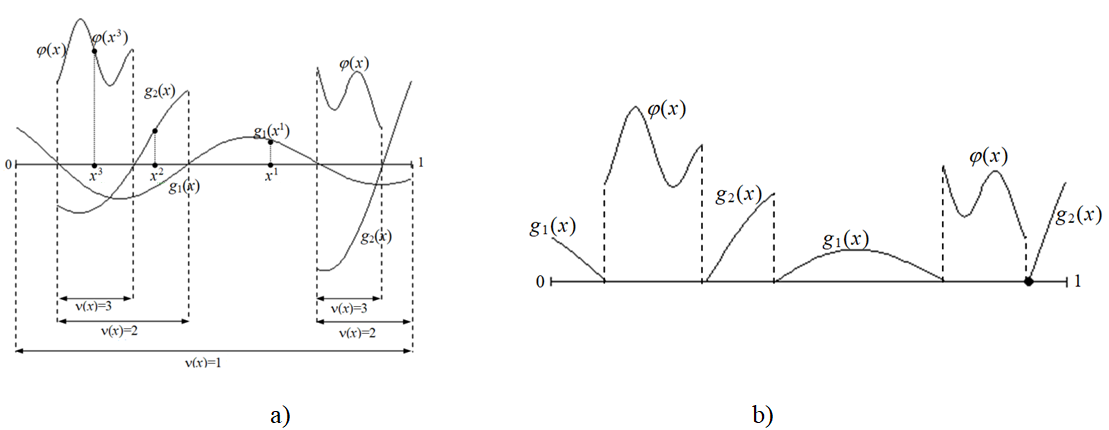
\includegraphics[width=\linewidth]{fig1}
  \caption{An example of the integrated function for the problem (\ref{eq:16}) using a sequential constraint calculation scheme: a) the initial problem functions, b) the function $F(x)$ from (\ref{eq:19})}
  \label{fig:1}
\end{figure}

The function $F(x)$ consists of separate fragments of the constraints ${g_i(x) \leq 0}$, $1 \leq i \leq m$, and the minimized function $\varphi(x)$. For the homogeneity of the components, the function $F(x)$ is converted to the form 
\begin{equation}\label{eq:20}
\Phi (x) = 
 \begin{cases}
   g_\nu(x) / H_\nu, & \nu < M, \\
   (g_M(x)-z^*_M) / H_M, & \nu = M,
 \end{cases}
\end{equation}
where $M$ is the constraint number, for which there are no feasible points (the maximum value of the index $\nu(x)$), $z^*_M$ is the value of the minimum constraint violation $g_M(x)$\footnote{If $M=m+1$, then $z_M^*$ is the minimum value of the function $\varphi(x)$.}, and $H_\nu$, $1\leq \nu \leq M$, are the H\"older constants from (\ref{eq:13}). As a rule, these values are a priori unknown, but when performing calculations, instead of these values, their adaptive estimates can be applied. For this, the search information $A_k$ from (\ref{eq:14}) should be expanded with data
\begin{equation}\label{eq:21}
A_k=\{(x_i, z_i, \nu_i, y(x_i), f_i=f(y(x_i))): 1 \leq i \leq k \},
\end{equation}
where $z_i= \Phi(x_i)$, $1 \leq i \leq k$. Then the estimates of the required values can be determined as follows
\begin{equation}\label{eq:22}
M^k = \max{\{\nu=\nu(x_i), 1\leq i \leq k \}},
\end{equation}

\begin{equation}\label{eq:23}
z^k_\nu = 
 \begin{cases}
   0, & \nu < M^k, \\
   \min{\{g_\nu(x_i):\nu=\nu(x_i), 1\leq i \leq k \}}, & \nu = M^k,
 \end{cases}
\end{equation}

\begin{equation}\label{eq:24}
H^k_l=\max{\{|z_i-z_j|/\sqrt[N]{x_i-x_j}, \nu_i=\nu_j=l, i>j, 1\leq l\leq M^k\}}.
\end{equation}

If $H_l^k$ in (\ref{eq:24}) turns out to be indefinite or equal to zero, then $H_l^k=1$ is taken. For the initial values of these parameters, $M^0 = H_l^0 = 1$, $z_l^0 = 0$, $1 \leq i \leq m+1$, can be taken.

In the framework of the proposed approach to minimize the function $\Phi(x)$, the global search algorithm for multiextremal optimization problems with nonlinear constraints\footnote{This method is also known as the index method -- see \cite{c18}.} (AGCS) is applied. The general computational scheme of this method can be presented as follows \cite{c18}.

The first trial is carried out at an arbitrary internal point $x^1\in(0,1)$. The choice of the point $x^{k+1}$, $k \geq 1$, of any next trial is determined by the following rules.

\textit{Rule 1.} For each interval $(x_{i-1},x_i)$, $1 < i \leq k$, in the set $A_k$ calculate the characteristic

\begin{equation}\label{eq:25}
R(i)=\mathcal{R} (i,A_k),
\end{equation}
where the expression $\mathcal{R}(i,A_k)$ is set by AGCS.

\textit{Rule 2.} Determine the interval $(x_{t-1},x_t)$ that corresponds to the maximum characteristic
\begin{equation}\label{eq:26}
R(t) = \max{\{R(i):1 < i \leq k\}}.
\end{equation}

\textit{Rule 3.} Execute a new trial at the point $x^{k+1} \in (x_{t-1},x_t)$, determined in accordance with the expression
\begin{equation}\label{eq:27}
x^{k+1} = \mathcal{X}(x_{t-1},x_t),
\end{equation}
where the expression $\mathcal{X}(x_{t-1},x_t)$ is also set by AGCS.

Iterations of the algorithm are terminated if the stop criterion is satisfied
\begin{equation}\label{eq:28}
\rho_t\leq \varepsilon,
\end{equation}
where $t$ from (\ref{eq:26}), $\rho_t = \sqrt[N]{x_t-x_{t-1}}$ and $\varepsilon > 0$ is the given accuracy.

Results of the application of the AGCS algorithm to solve the test problem from Fig.~\ref{fig:1} with the accuracy $\varepsilon=10^{-5}$ are shown in Fig.~\ref{fig:2}. The coordinates of the trial points performed by the algorithm in the process of solving the problem are marked in Fig.~\ref{fig:2} by three rows of vertical strokes. The strokes in the upper row correspond to points with a unit index, the second row to points, the indices of which equal to $\nu=2$; the points marked with strokes in the bottom row belong to the feasible domain. The coordinates of trials performed at close points are marked with a dark rectangle. In total, the value of the first constraint was computed 147 times, the value of the second constraint -- 84 times, and the value of the minimized function was calculated only 35 times.

\begin{figure}
  \centering
  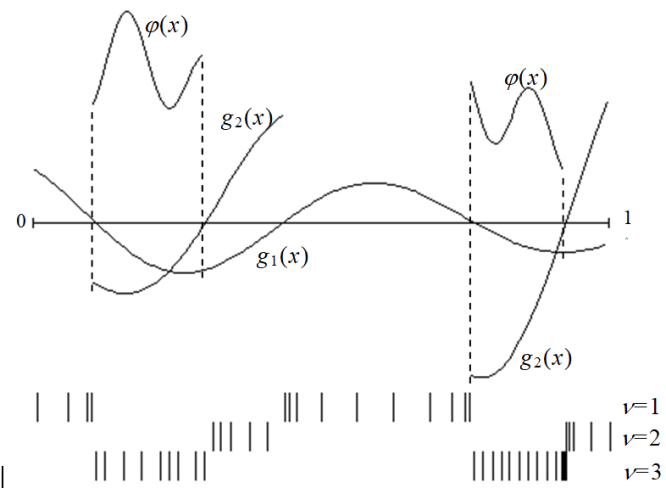
\includegraphics[width=0.6\linewidth]{fig2}
  \caption{Results of using the AGCS algorithm to solve the test problem}
  \label{fig:2}
\end{figure}

Various modifications of this algorithm and the corresponding theory of convergence are presented in \cite{c18}.
In particular, one modification of the algorithm involves using information about local behavior of the problem functions \cite{Sergeyev2003}.

The AGCS convergence conditions are defined by the following theorem from  \cite{c18}.

\begin{theorem}
If the AGCS algorithm is used to solve the problem (\ref{eq:16}), and the following conditions are satisfied:
\begin{enumerate}
	\item the functions $g_j(x)$, $1 \leq j \leq m+1$, $x\in[0,1]$, satisfy the H\"older condition with the constants $H_j$, $1 \leq j \leq m+1$,
	\item for the values $H^k_\nu$ from (\ref{eq:24}), starting from a certain step, the inequalities are valid\footnote{The values $r_{\nu} > 1$, $1 \leq \nu \leq m+1$, are the AGCS reliability parameters used for computing the interval characteristics in (\ref{eq:25}).}
\begin{equation} \label{eq:29}
r_\nu H^k_\nu > 2H_\nu, r_\nu > 1, 1 \leq \nu \leq m+1,
\end{equation}
\end{enumerate}
then the set of limit points of the sequence $\{x^k\}$ generated by the algorithm coincides with the set of global minimum points of the problem (\ref{eq:16}) with $\varepsilon=0$ in the stopping criterion (\ref{eq:28}).
\end{theorem}

\subsection{Acceleration of Computations Based on the Reuse of Search Information}

As noted earlier, the MCOlex problem at each stage (\ref{eq:9}) of the $\varepsilon$-constraint method is a global optimization problem with nonlinear constraints (\ref{eq:16}). Generally, the solution to such problems should start from the very beginning; and multiple solutions to such global optimization problems may require extensive calculations. However, the presence of search information $A_k$ from (\ref{eq:21}) allows bringing the results of previous calculations to the values of any next solved optimization problem in the scheme (\ref{eq:9}) without any time-consuming calculations of the values of the criteria $f_j (y)$, $1 \leq j \leq s$, of the problem (\ref{eq:1}) \cite{c30,c31}. 
The search information can be reused by using the algorithm briefly described below.
\begin{itemize}
\item 
When the criterion $f_j(y(x)), 1\leq j\leq s,$ is minimized, the resulting search information is accumulated as a set $A_k$ from (\ref{eq:21}) (note that along with the values $z_i, 1\leq i\leq k,$ of the minimized criterion $f_j(y(x))$, $A_k$ also accumulates the calculated values of the vector criterion $f(y(x_i)), 1\leq i\leq k$).
\item 
When the minimization of the next criterion $f_{j+1}(y(x))$ begins, the values of this criterion $z'_i, 1\leq i\leq k,$ at all the points  $x_i, 1\leq i\leq k,$ of the previously completed iterations of the global search can be obtained via quick calculations based on the stored values of the vector criterion $f(y(x_i)), 1\leq i\leq k,$ in the search information $A_k$
\begin{equation}\label{new_equation}
z'_i=Z(f(y(x_i))), 1\leq i\leq k,
\end{equation}
where calculation procedure of the values $z'_i, 1\leq i\leq k$ is determined by the rules (\ref{eq:9}), (\ref{eq:18})--(\ref{eq:20}), without any need to repeat calculations of criteria values $f_j(y(x)), 1\leq l\leq s$.
\end{itemize}

This reuse of search information to find the next efficient decision reduces the number of computations needed to solve each next optimization problem to just a few iterations -- see Section \ref{sec:5} for the results of numerical experiments.

Moreover, using the search information $A_k$ allows reducing the multistage solution of the MCOlex problem in accordance with the scheme (\ref{eq:9}) to the solution of the only global optimization problem in the last stage of the scheme (\ref{eq:9}), namely
\begin{equation}\label{eq:30}
P_{\delta lex} (f,\delta,D)=\arg \min_{y \in D} { \{ f_s(y), f_j(y)\leq f_j^* + \delta_j, 1 \leq j < s\} },
\end{equation}
where for the unknown a priori values $f_j^*$, $1 \leq j < s$, the estimates $z_j^k$, ${1 \leq j < s}$, from (\ref{eq:23}) obtained from the search information $A_k$ can be used, and for the concessions $\delta_j$, $1 \leq j < s$, the normalized values can be applied, that is
\begin{equation}\label{eq:31}
	\begin{matrix}
	\delta_j = z_j^k + \theta_j (g_j^k-z_j^k ), 0 \leq \theta_j \leq 1, 1 \leq j < s,\\
	g_j^k = \max{\{ g_j (x_i ) : \nu(x_i)=j, 1 \leq i \leq k \}}.
	\end{matrix}
\end{equation}
Considering this and previous examples, when any changes in estimates $f_j^*, \delta_j,$ $g_j^k, 1\leq j < s, 1 \leq i \leq k,$ occur, the solution of the problem (\ref{eq:30}) can be continued using all the available search information after the new values $z'_i,1\leq i \leq k,$ are promptly calculated following the procedure (\ref{new_equation}).
In particular, a similar one-step scheme (\ref{eq:30})--(\ref{eq:31}) can be applied through the use of AGCS.

With a complete scheme for calculating criteria values, i.e. when at the iteration points $x_i$, $1 \leq i \leq k$, the values of all criteria $f_j(x_i)$, $1 \leq j \leq s$, $1 \leq i \leq k$, are calculated, the effect of using the search information $A_k$ can be even more significant. In this case, the search information can also be used when changing the values of the concessions $\delta_j$, $1 \leq j < s$, and thus, the solution of the next problem from the $\mathbb{F}$ family (\ref{eq:10}) can be carried out repeatedly using the results of all previously performed calculations. The results of numerical experiments (see Section \ref{sec:5}), demonstrate that the volume of computations performed, based on reusing search information, can significantly decrease.

The AGCS algorithm, supplemented by the ability to use search information to solve MMCOlex problems, will be referred to below as the global search algorithm for multistage solutions of a set of multiextremal optimization problems with nonlinear constraints (MAGCS).

\section{Evaluation of the Effectiveness of Search Information Reuse}
\label{sec:4}

Evaluation of the effectiveness of multiple uses of search information is based on the key properties of the AGCS algorithm. When searching for the global minimum, this algorithm constructs a grid of search trial points covering the search domains. In addition, this algorithm is stable, i.e., in minor variations of the minimized function, the value of change in the evaluation of the global minimum is limited.

To reduce the complexity of theoretical analysis, all further studies have been performed for the one-dimensional version of the AGCS algorithm; due to the use of dimensional reduction, the results obtained will also be applicable when solving multidimensional optimization problems.

The initial theoretical analysis of global search properties when using search information was performed in \cite{c31}. The obtained theoretical statements can be reformulated as applied to lexicographic multicriteria optimization problems. 


\begin{theorem}
Let the next minimized function $\psi(x)$ of the computational scheme (\ref{eq:9}) differ from the previous minimized function $\phi(x)$ by some limited value $\delta$, i.e.
\begin{equation}\label{eq:32}
|\psi(x)-\phi(x)| \leq \delta, x \in [0,1],
\end{equation}
and let the stopping criterion of (\ref{eq:28}) for the specified accuracy of global search $\varepsilon>0$ be fulfilled when minimizing the function $\phi(x)$. Then 
\begin{equation}\label{eq:33}
|\psi(x^*)-\phi(x_k^*)| \leq \Delta = \frac{\alpha L \varepsilon}{2} + \delta,
\end{equation}
if starting from a certain iteration $k_0>0$ the condition is fulfilled for the estimation of the Lipschitz constant $m$ and some $\alpha > 1$
\begin{equation}\label{eq:34}
m \geq L (1+ \sqrt{\frac{\alpha + 4 \beta (1 + \beta)}{\alpha - 1}}),
\end{equation}
where
\begin{equation}\label{eq:35}
m=\max{\{r_l H_l^k, 1 \leq l \leq M^k \} }, k>k_0,
\end{equation}
\begin{equation}\label{eq:36}
L=\max{\{L_i, 1 \leq i \leq s \}}, \; L_i\; \text{from}\; (\ref{eq:3}),
\end{equation}
\begin{equation}\label{eq:beta}
\beta =  \frac{2r\delta} {L\varepsilon(r-1)},
\end{equation}
\begin{equation}\label{eq:37}
\psi(x^*)=\min{\{\psi(x), x \in [0,1]\}},
\end{equation}
\begin{equation}\label{eq:38}
x_k^* = \arg \min{\{\phi(x_k), 1 \leq i \leq k\}}.
\end{equation}
\end{theorem}
The points $x_k$, $1 \leq i \leq k$, in (\ref{eq:38}) are taken from search information $A_k$ from (\ref{eq:21}) obtained by minimizing the function $\phi(x)$, and $H_l^k$, $M^k$, $r_l$ are the values of (\ref{eq:22}), (\ref{eq:24}) and (\ref{eq:29}), respectively.

This statement means that if the error $\Delta$ from (\ref{eq:33}) of determination of the minimum value of $\psi(x^*)$ is acceptable, then the minimization of the function $\psi(x)$ does not require any additional iterations of the global search -- the evaluation of the minimum value of $\psi(x^*)$ can be obtained in accordance with (\ref{eq:33}), using values $x_k$, ${1 \leq i \leq k}$, located in the search information $A_k$ from (\ref{eq:21}), obtained by minimizing the function $\phi(x)$.

\begin{theorem}
Let the function $\phi(x)$ of the computational scheme (\ref{eq:9}) be minimized before the stopping criterion in (\ref{eq:28}) is fulfilled for the specified accuracy of the global search $\varepsilon > 0$ and the density of trials $p_{ab}$ for the interval $[a,b] \subset [0,1]$ is reached
\begin{equation}\label{eq:39}
p_{ab}=\frac{n_{ab}}{b-a},
\end{equation}
where $n_{ab}$ is the number of trial points in the interval $[a,b]$ during the minimization of the function $\phi(x)$. Then, when minimizing the next function $\psi(x)$ using the search information $A_k$ from (\ref{eq:21}) obtained by minimizing the function $\phi(x)$, the number of trials in the same interval $[a,b]$ instead of the maximum value
\begin{equation}\label{eq:40}
(3m/2\Delta)(b-a), \text{where} \; m \; \text{is from} \;  (\ref{eq:35}),
\end{equation}
will be limited by the value
\begin{equation}\label{eq:41}
n_{ab}' \leq (3m/2\Delta - p_{ab})(b-a)
\end{equation}
if the condition is met
\begin{equation}\label{eq:42}
\psi(x) \geq \psi(x^*)+\Delta, x \in [a,b].
\end{equation}
\end{theorem}

Considering the estimate (\ref{eq:41}) of the maximum number of trials in the search domain subintervals $[0,1]$, the following statement may be formulated.

\begin{theorem}
If the number of trials in the interval $[a,b]\subset[0,1]$ exceeds the maximum estimate (\ref{eq:41}) when minimizing the function $\phi(x)$ of the computational scheme (\ref{eq:9}), then when minimizing the next function $\psi(x)$ using the search information $A_k$ from (\ref{eq:21}) obtained by minimizing the function $\phi(x)$, additional trials in the interval $[a,b]$ will not be performed while the condition (\ref{eq:42}) is fulfilled.
\end{theorem}

The theoretical statements formulated above allow estimating the positive effect of multiple uses of search information obtained in the process of calculations. If the new problem is sufficiently close to the already solved problems, the evaluation of the global search can be obtained based on the available search information without performing additional iterations of the global search (Theorem 2). In the extreme case, when solving a sufficient number of information-connected optimization problems, each new problem can be close to one of the previously solved problems, making the already available search information sufficient for solving this new problem. In other cases, when a new optimization problem is quite different from the previously solved problems, the use of search information, previously obtained in the course of calculations, allows reducing the number of trials performed in the subintervals of the search domain $[0,1]$ up to the complete absence of additional trials in these subintervals (Theorems 3-4).

\section{Results of Numerical Experiments}
\label{sec:5}

The numerical experiments were carried out on the Lobachevsky supercomputer at the Lobachevsky State University of Nizhny Novgorod (the CentOS 6.4 operating system and the SLURM workload manager). A supercomputer node has 2 Intel Sandy Bridge E5-2660 2.2 GHz, 64 Gb RAM processors. Each CPU is 8-core, which means 16 CPU cores are available on the node. The Intel C ++ 14.0.2 compiler was used to obtain an executable program code. The numerical experiments were performed using the Globalizer system \cite{c32}.

Evaluating the efficiency of multicriteria optimization methods is not quite a trivial question. While the efficiency of scalar optimization methods can be evaluated by the indicators of solution accuracy and the number of optimization iterations performed (the number of the calculated function values), solving MCO problems can lead to finding several efficient decisions or even approximating the whole Pareto set. There are many different approaches to this issue -- for example, efficiency indicators can be determined by the mutual domination rate \cite{c49}, the degree of approximation \cite{c50}, the overall Pareto spread \cite{c51}, etc. Authors of \cite{c52} propose an even wider set of 57 efficiency indicators in solving MCO problems. Unfortunately, it should be noted that no single approach has yet been adopted to evaluate the efficiency of the MCO methods. 

In this paper we assessed the efficiency of the MCO methods using two widely used indicators \cite{c35,c36}:
\begin{itemize}
	\item The hypervolume index (HV). This indicator evaluates the approximation of the Pareto set in terms of completeness; a higher value corresponds to a more complete coverage of the Pareto set.
	\item The distribution uniformity index (DU). This indicator evaluates the uniformity of Pareto set coverage; a lower value corresponds to a more uniform coverage of the Pareto set.
\end{itemize}

In addition, since the solution of the MCO problem is reduced to the solution of multiple scalar optimization problems, the efficiency will be evaluated by ``classical'' indicators: the solution accuracy and the number of the calculated function values. The latter indicator is even more important because due to the initial assumption about the time-consuming calculations of efficiency criteria values of the MCO problem, this indicator evaluates the computational complexity of solving the MCO problem.

Another important issue of the efficiency evaluation consists in the choice of benchmarks, which will be used to measure the efficiency of the methods applied. Unfortunately, there is no unified approach to this issue either. In many studies, the efficiency of the developed methods is demonstrated by the example of a limited set of test optimization problems. Researchers repeatedly attempt to resolve this issue by forming quite a wide set of test optimization problems, which can be used to evaluate the efficiency of the MCO methods. For instance, in \cite{c53} authors propose a flexible toolkit for constructing well-designed MCO problems. In \cite{c54} a set of 24 test optimization functions is given, which are widely used for evaluating the MCO methods. In \cite{c55} a set of 100 test problems is considered. In \cite{c56} an approach is proposed, in which a set of efficiency criteria of the MCO problems is formed from the well-known scalar optimization functions. This allows forming an almost endless set of MCO problems. At the same time, the set of the MCO test problems, in which the efficiency criteria would be multiextremal functions, is rather limited. Also, the proposed sets usually consist of single examples of the MCO problems, which makes it difficult to obtain any reliable estimates of the method efficiency. 

In this paper, the efficiency of the proposed methods is evaluated by executing extensive numerical experiments for solving the wide sets of the MCO problems. The test problems are produced by the GKLS generator \cite{c37} that can construct an almost endless number of the MCO problems using a random mechanism. This generator can produce multiextremal functions with predetermined characteristics (the dimensionality, the number of local minima, the size of their attraction domains, the point of global minimum, and the value of the functions, etc.). Fig. \ref{fig:3} shows an example of the two criteria generated using GKLS.

\begin{figure}
  \centering
  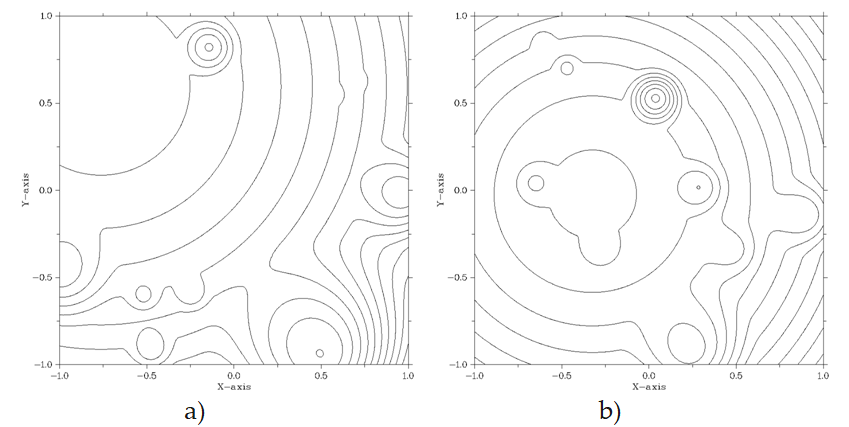
\includegraphics[width=0.8\linewidth]{fig3}
  \caption{Contour plots of two criteria obtained by the GKLS generator}
  \label{fig:3}
\end{figure}

As we have previously noted, the proposed global optimization algorithms were developed in the framework of the information-statistical theory of multiextremal optimization. These methods have proven to be efficient in numerical experiments and have been widely used for solving practical global optimization problems (see, e.g., \cite{c17,c18,c23,c26,c27,c33,c34}). The results of numerical experiments in solving multicriteria optimization problems are given below.

In the first series of numerical experiments, the MAGCS algorithm was compared with several multicriteria optimization algorithms for solving the two-criteria problem proposed in \cite{c35}:
\begin{equation}\label{eq:43}
f_1 (y)=(y_1-1) y_2^2+1,f_2 (y)=y_2, 0\leq y_1,y_2 \leq 1.
\end{equation}

In this experiment, five multicriteria optimization algorithms were compared: the Monte-Carlo (MC) method, the genetic algorithm SEMO from the PISA library \cite{c9,c36}, the Non-uniform coverage (NUC) method \cite{c35}, the bi-objective Lipschitz optimization (BLO) method \cite{c36}, and the MAGCS algorithm. The results of the solution (\ref{eq:29}) for all these methods (except for MAGCS) were obtained in \cite{c36}.

For MAGCS, the problem (\ref{eq:43}) is considered as the MMCOlex problem, which includes 50 subproblems (\ref{eq:30}) with different values
$\theta_1$ from (\ref{eq:31}), uniformly distributed in the interval $[0,1]$. The accuracy $\varepsilon=0.05$ from (\ref{eq:28}) and the reliability parameters $r_1=r_2=3.0$ from (\ref{eq:29}) were used. The results of the executed experiments are presented in Table \ref{tab:1}.


\begin{table}[ht]
\centering
\caption{The numerical results of solving the multicriteria optimization problems from (\ref{eq:43})}
\label{tab:1}
\begin{tabular}{cccccc}
\hline
Method                                                                                     & MC    & SEMO  & NUC   & BLO   & \textbf{MAGCS} \\ \hline
Number of executed iterations                                                              & 500   & 500   & 515   & 498   & \textbf{273}   \\
\begin{tabular}[c]{@{}c@{}}Number of points in \\ the Pareto set approximation\end{tabular} & 67    & 104   & 29    & 68    & \textbf{80}    \\
HV index                                                                                   & 0.300 & 0.312 & 0.306 & 0.308 & \textbf{0.314} \\
DU index                                                                                   & 1.277 & 1.116 & 0.210 & 0.175 & \textbf{0.096} \\ \hline
\end{tabular}
\end{table}

The results of the executed experiments demonstrate that the MAGCS algorithm has a significant advantage in comparison with the considered multicriteria optimization methods, even when solving relatively simple MCO problems.



All the subsequent numerical experiments focused on the solution of 
the MMCOlex problems, which includes 100 two-criteria MCO problems, the efficiency criteria of which were set by the GKLS generator.
Each MCO problem from the generated set is considered as the MMCOlex problem, which includes from 10 to 100 subproblems (\ref{eq:30}) with different
values $\theta_1$ from (\ref{eq:31}), uniformly distributed in the interval $[0,1]$. The obtained results of numerical experiments were averaged by the number of solved MCO problems. 

The solution of MCOlex problems was carried out before the stopping criterion of (\ref{eq:28}) was fulfilled, and the MCOlex problems were considered solved correctly if the distance of the solutions to the Pareto set did not exceed the given accuracy $\varepsilon$ from (\ref{eq:28}).
 
In the second series of experiments, the two-criteria two-dimensional MCO problems were solved. The solution was carried out with the method accuracy $\varepsilon = 0.025$ and the reliability parameters $r_1 = r_2 = 5.6$. The results of numerical experiments are presented in Table \ref{tab:2}.


\begin{table}[ht]
\centering
\caption{Results of the numerical experiments to solve two-criteria two-dimensional MCO problems}
\label{tab:2}
\resizebox{\columnwidth}{!}{%
\begin{tabular}{cccccccccccc}
\hline
    & \multicolumn{10}{c}{Solving   MCO problems}                                                             &     \\ \cline{2-11}
SP  & \multicolumn{5}{c}{without   using search information} & \multicolumn{5}{c}{using   search information} & RI  \\ \cline{2-11}
    & PI          & SPI      & SPS       & HV       & DU     & PI        & SPI    & SPS      & HV     & DU    &     \\ \hline
10  & 8 340,1     & 834,0    & 71,3\%    & 30,34    & 0,35   & 981,7     & 98,2   & 81,9\%   & 30,10  & 0,54  & 1,0 \\
20  & 16 756,5    & 837,8    & 78,0\%    & 30,56    & 0,31   & 1 208,0   & 60,4   & 86,8\%   & 30,25  & 0,42  & 1,6 \\
30  & 25 209,4    & 840,3    & 80,7\%    & 30,60    & 0,32   & 1 319,2   & 44,0   & 89,7\%   & 30,33  & 0,45  & 2,2 \\
40  & 33 625,7    & 840,6    & 81,7\%    & 30,65    & 0,31   & 1 403,0   & 35,1   & 92,4\%   & 30,40  & 0,40  & 2,8 \\
50  & 41 994,7    & 839,9    & 82,8\%    & 30,68    & 0,31   & 1 452,8   & 29,1   & 93,5\%   & 30,46  & 0,41  & 3,4 \\
60  & 50 428,8    & 840,5    & 83,5\%    & 30,72    & 0,29   & 1 506,6   & 25,1   & 93,8\%   & 30,46  & 0,37  & 3,9 \\
70  & 58 923,3    & 841,8    & 84,5\%    & 30,75    & 0,29   & 1 556,9   & 22,2   & 95,1\%   & 30,52  & 0,37  & 4,4 \\
80  & 67 318,8    & 841,5    & 84,8\%    & 30,76    & 0,30   & 1 588,5   & 19,9   & 95,3\%   & 30,51  & 0,38  & 4,9 \\
90  & 75 684,0    & 840,9    & 85,0\%    & 30,76    & 0,25   & 1 624,7   & 18,1   & 95,5\%   & 30,57  & 0,37  & 5,4 \\
100 & 84 164,2    & 841,6    & 84,6\%    & 30,78    & 0,26   & 1 644,3   & 16,4   & 95,9\%   & 30,58  & 0,32  & 6,0 \\ \hline
\end{tabular}
}
\end{table}

The first column (SP) in the Table \ref{tab:2} contains the total number of MCOlex subproblems to be solved. The PI columns show the average number of iterations for solving one MCO problem. The SPI columns represent the average number of iterations for solve a single MCOlex subproblem. The SPS columns contain a fraction of MCOlex subproblems solved with the required accuracy. The HV and DU columns show the hypervolume (HV) and the distribution uniformity (DU) indices of the calculated approximation of the Pareto set, respectively. The last column (RI) shows the degree of the reduction in the number of global search iterations performed when solving subproblems (\ref{eq:30}) by reusing the search information.

The results presented in Table \ref{tab:2} demonstrate that the use of search information allows to obtain an estimate of the Pareto set after a substantially smaller total number of iterations of the global search (the PI columns). It should also be noted that as the number of solved subproblems increases, the MAGCS allows to build estimates of the Pareto set with better HV and DU indices.

For a better visual representation, Fig. \ref{fig:4} shows the average number of iterations performed to solve a single MCOlex subproblem with and without search information. The presented graphs convincingly demonstrate a significant reduction in the number of global search iterations when solving the MCOlex subproblems using search information.

\begin{figure}
  \centering
  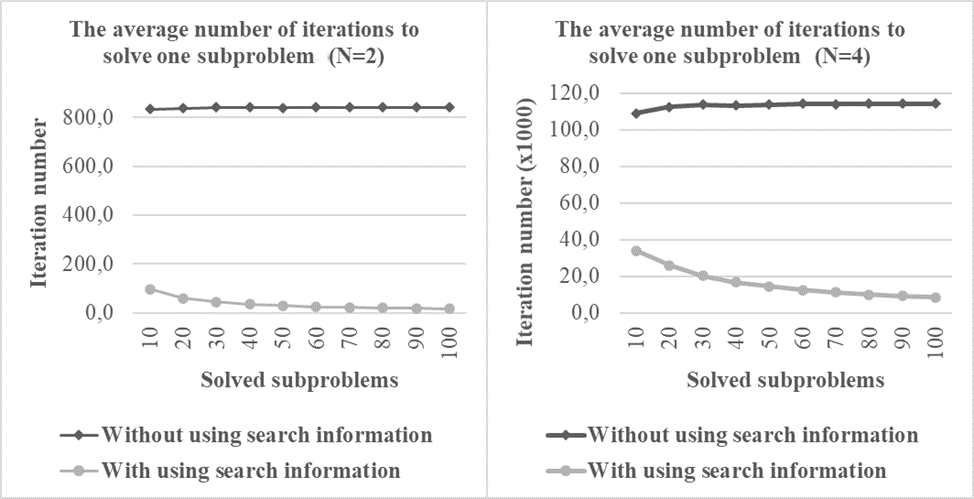
\includegraphics[width=1\linewidth]{fig4}
  \caption{Average number of iterations required to solve one MCOlex subproblem depending on the total number of subproblems solved}
  \label{fig:4}
\end{figure}

Fig. \ref{fig:5} shows the reduction in the number of global search iterations when solving MCOlex subproblems using search information. The graphs presented show that when the number of solved MCOlex subproblems grows linearly, the number of iterations required to solve one subproblem is reduced almost linearly as well.

\begin{figure}
  \centering
  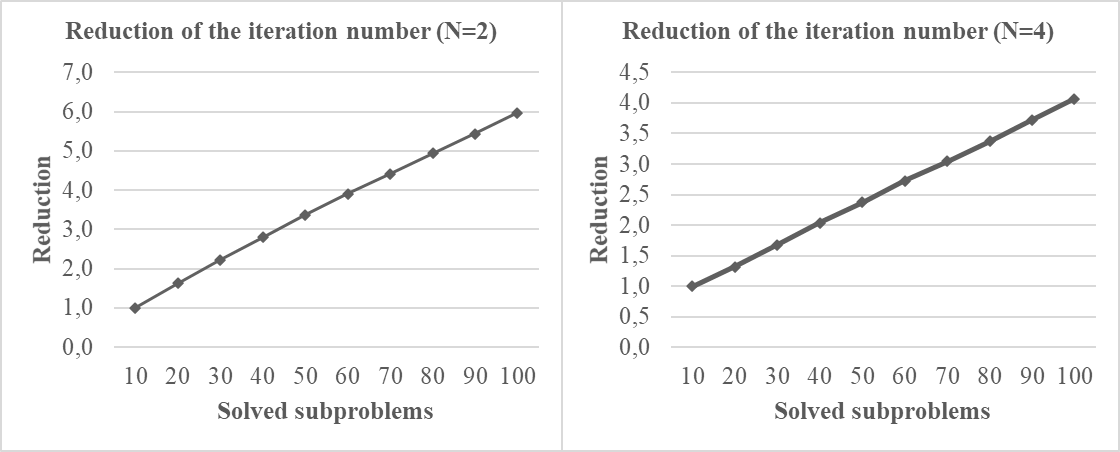
\includegraphics[width=1\linewidth]{fig5}
  \caption{Reduction of the number of iterations performed to solve one MCOlex subproblem depending on the total number of subproblems solved}
  \label{fig:5}
\end{figure}

It should be noted that the number of global search iterations is also reduced in the course of sequential solution of the subproblems of the same MCO problem. Table \ref{tab:3} illustrates this trend showing the average number of iterations required to find a solution to one MCOlex subproblem, with subdividing the sequence of solved subproblems in groups of 10 MCOlex subproblems. The first row (SP) contains the MCOlex subproblem numbers belonging to the individual subproblem groups. The PI rows show the total number of iterations of the global search performed for all previous problems. The rows labeled as ``PI new'' show the number of iterations performed to solve the next group of MCOlex subproblems with the numbers of the problems given in each column heading. The last row labeled as ``FPI new'' shows the proportion of new iterations of global search performed to solve the next group of MCOlex subproblems.

\begin{table}[ht]
\centering
\caption{Average number of iterations to solve two-criteria two-dimensional MCO problems}
\label{tab:3}
\resizebox{\columnwidth}{!}{%
\begin{tabular}{ccccccccccc}
\hline
SP       & 1-10   & 11-20  & 21-30  & 31-40  & 41-50  & 51-60  & 61-70  & 71-80  & 81-90  & 91-100 \\ \hline
\multicolumn{11}{c}{Solving MCO problems without using search information}                         \\ \hline
PI       & 8868   & 17007  & 26228  & 34320  & 44117  & 53776  & 63292  & 71816  & 78824  & 84164  \\
PI new   & 8868   & 8139   & 9221   & 8092   & 9796   & 9660   & 9515   & 8525   & 7007   & 5341   \\ \hline
\multicolumn{11}{c}{Solving MCO problems with using search information}                            \\ \hline
PI       & 993,1  & 1230,3 & 1309,6 & 1393,2 & 1409,5 & 1430,9 & 1466,1 & 1538,2 & 1624,9 & 1644,3 \\
PI new   & 993,1  & 237,1  & 79,3   & 83,6   & 16,3   & 21,4   & 35,2   & 72,1   & 86,7   & 19,4   \\ \hline
\multicolumn{11}{c}{Proportion of new iterations   for the solution of a new group of subproblems} \\ \hline
FPI new  & -      & 23,9\% & 6,4\%  & 6,4\%  & 1,2\%  & 1,5\%  & 2,5\%  & 4,9\%  & 5,6\%  & 1,2\%  \\ \hline
\end{tabular}
}
\end{table}

Fig. \ref{fig:6} shows the values of the achieved reduction in the number of additional iterations required to solve the next set of subproblems (the last row of Table \ref{tab:3}). The above data demonstrates that solving the next group of MCOlex subproblems requires about $6\%$ of new global search iterations in addition to the available search information.

\begin{figure}
  \centering
  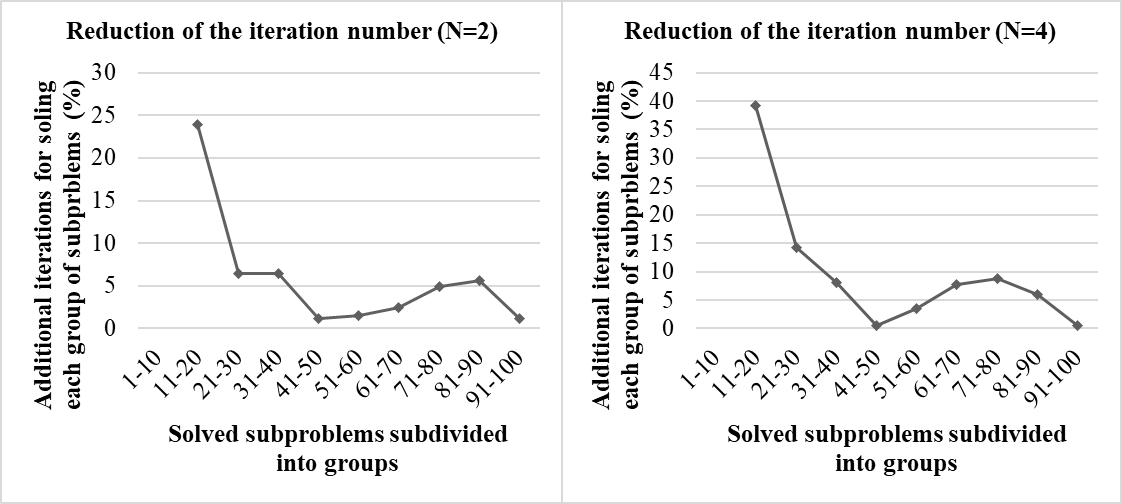
\includegraphics[width=1\linewidth]{fig6}
  \caption{Proportion of new global search iterations for solving the next group of MCOlex subproblems}
  \label{fig:6}
\end{figure}

The third set of numerical experiments was designed to demonstrate the scalability of the proposed approach by solving more complex two-criteria four-dimensional MCO problems under the same conditions as in the previous series of calculations. The results of the experiments are presented in Tables \ref{tab:4}--\ref{tab:5} and in Fig. \ref{fig:4}--\ref{fig:6}. These data demonstrate that the experiments carried out to solve more complex MCO problems confirm the conclusions made earlier -- for example, solving the next group of MCOlex subproblems requires, in addition to the available search information, from $0.5\%$ to $14.2\%$ more global search iterations (Table \ref{tab:5}, last row).


\begin{table}[ht]
\centering
\caption{Results of the numerical experiments to solve two-criteria four-dimensional MCO problems}
\label{tab:4}
\resizebox{\columnwidth}{!}{%
\begin{tabular}{cccccccccccc}
\hline
    & \multicolumn{10}{c}{Solving MCO problems}                                                                &     \\ \cline{2-11}
SP  & \multicolumn{5}{c}{without using search information} & \multicolumn{5}{c}{With using search information} & RI  \\ \cline{2-11}
    & PI$\times 10^3$& SPI$\times 10^3$& SP       & HV      & DU     & PI$\times 10^3$& SPI$\times 10^3$& SP       & HV      & DU    &     \\ \hline
10  & 1 088,7    & 108,8     & 71,3\%   & 30,34   & 0,35   & 340,4    & 34,0      & 81,9\%   & 30,10   & 0,54  & 1,0 \\
20  & 2 245,6    & 112,2     & 78,0\%   & 30,56   & 0,31   & 518,3    & 25,9      & 86,8\%   & 30,25   & 0,42  & 1,3 \\
30  & 3 407,8    & 113,5     & 80,7\%   & 30,60   & 0,32   & 607,9    & 20,2      & 89,7\%   & 30,33   & 0,45  & 1,7 \\
40  & 4 525,3    & 113,1     & 81,7\%   & 30,65   & 0,31   & 669,6    & 16,7      & 92,4\%   & 30,40   & 0,40  & 2,0 \\
50  & 5 677,0    & 113,5     & 82,8\%   & 30,68   & 0,31   & 717,2    & 14,3      & 93,5\%   & 30,46   & 0,41  & 2,4 \\
60  & 6 854,4    & 114,2     & 83,5\%   & 30,72   & 0,29   & 750,3    & 12,5      & 93,8\%   & 30,46   & 0,37  & 2,7 \\
70  & 7 965,3    & 113,7     & 84,5\%   & 30,75   & 0,29   & 782,3    & 11,1      & 95,1\%   & 30,52   & 0,37  & 3,0 \\
80  & 9 134,8    & 114,1     & 84,8\%   & 30,76   & 0,30   & 807,4    & 10,0      & 95,3\%   & 30,51   & 0,38  & 3,4 \\
90  & 10 280,2   & 114,2     & 85,0\%   & 30,76   & 0,25   & 822,7    & 9,1       & 95,5\%   & 30,57   & 0,37  & 3,7 \\
100 & 11 401,9   & 114,0     & 84,6\%   & 30,78   & 0,26   & 836,3    & 8,3       & 95,9\%   & 30,58   & 0,32  & 4,1 \\ \hline
\end{tabular}
}
\end{table}

\begin{table}[ht]
\centering
\caption{Results of the numerical experiments to solve two-criteria four-dimensional MCO problems}
\label{tab:5}
\resizebox{\columnwidth}{!}{%
\begin{tabular}{ccccccccccc}
\hline
SP          & 1-10   & 11-20  & 21-30  & 31-40  & 41-50  & 51-60  & 61-70  & 71-80  & 81-90   & 91-100  \\ \hline
\multicolumn{11}{c}{Solving MCO problems without using   search information}                            \\ \hline
PI$\times 10^3$& 1167,1 & 2320,4 & 3403,4 & 4530,1 & 5543,4 & 6603,5 & 7968,0 & 9614,4 & 10832,6 & 11402,0 \\
PI new$\times 10^3$& 1167,1 & 1153,3 & 1083,0 & 1126,7 & 1013,3 & 1060,1 & 1364,5 & 1646,4 & 1218,2  & 569,4   \\ \hline
\multicolumn{11}{c}{Solving MCO problems with using   search information}                               \\ \hline
PI$\times 10^3$& 399,5  & 556,1  & 635,1  & 686,1  & 690,3  & 714,4  & 769,4  & 837,3  & 886,7   & 890,7   \\
PI new$\times 10^3$& 399,5  & 156,6  & 79,0   & 51,0   & 4,2    & 24,2   & 54,9   & 67,9   & 49,4    & 4,0     \\ \hline
\multicolumn{11}{c}{Proportion   of new iterations required to solve the next group of subproblems}     \\ \hline
FPI new  & -      & 39,2\% & 14,2\% & 8,0\%  & 0,6\%  & 3,5\%  & 7,7\%  & 8,8\%  & 5,9\%   & 0,5\%   \\ \hline
\end{tabular}
}
\end{table}


\section{Conclusion}
\label{sec:6}

In this paper a new approach is proposed for solving computationally expensive lexicographic multicriteria optimization problems (MCOlex), which can be complicated by the multiextremal nature of the efficiency criteria and extensive volume of computations required to calculate the criteria values. A key feature of this class of problems is the ability to alter the ranking of efficiency criteria in terms of importance during calculations, which in turn necessitates a multistage solution for MCOlex problems. This new type of problems is referred to as MMCOlex problems.f

The computational complexity of addressing the formulated MMCOlex problems can be overcome by solving a sequence of global optimization problems with nonlinear constraints using efficient information-statistical methods of global optimization. A core element in this approach is the ability to use all the search information obtained in the course of solving the MMCOlex problems. With each new stage of the solution, this search information allows incorporating the previously calculated values of efficiency criteria into the values of the next scalar problem of multiextremal optimization. The search information retrieved becomes part of the current optimization state and, through optimization methods, results in adaptive planning of the iterations to run the global search. 

The results of numerical experiments demonstrate that this approach can sufficiently reduce the computational complexity of MMCOlex problem-solving.

In conclusion, it can be noted that the approach described here is promising, and requires further studies. It is necessary to continue numerical experiments to solve multicriteria optimization problems with a larger number of efficiency criteria and for greater dimensions in the optimization problems. It is also necessary to evaluate the possibility of parallel computing using high-performance supercomputer systems.



% Non-BibTeX users please use
\begin{thebibliography}{}
%
% and use \bibitem to create references. Consult the Instructions
% for authors for reference list style.
%

\bibitem{c1} Miettinen K.: Nonlinear Multiobjective Optimization. Springer. (1999)
\bibitem{c2} Ehrgott, M.: Multicriteria Optimization. Springer. (2nd ed., 2010)
\bibitem{c3} Collette, Y., Siarry, P.: Multiobjective Optimization: Principles and Case Studies (Decision Engineering). Springer. (2011)
\bibitem{c4} Marler, R.T., Arora, J.S.: Multi-Objective Optimization: Concepts and Methods for Engineering. VDM Verlag. (2009)
\bibitem{c5} Pardalos, P.M., {\v Z}ilinskas, A., {\v Z}ilinskas, J.: Non-Convex Multi-Objective Optimization. Springer. (2017)
\bibitem{c6} Marler, R., Arora , J.: Survey of multi-objective optimization methods for engineering. Struct. Multidisc. Optim. \textbf{26}, 369--395 (2004)
\bibitem{c7} Figueira,J., Greco, S., Ehrgott, M., (eds.): Multiple criteria decision analysis: State of the art surveys. Springer, New York (NY). (2005)
\bibitem{c8} Zavadskas, E.K., Turskis, Z., Kildien\.e, S.: State of art surveys of overviews on MCDM/MADM methods. Technol. Econ. Dev. Econ. \textbf{20}, 165--179 (2014)
\bibitem{c9} Hillermeier, C., Jahn, J.: Multiobjective optimization: survey of methods and industrial applications. Surv. Math. Ind. \textbf{11}, 1--42 (2005)
\bibitem{c14} Eichfelder, G.: Scalarizations for adaptively solving multi-objective optimization problems. Comput. Optim. Appl. \textbf{44}, 249--273 (2009)
\bibitem{c10} Branke, J., Deb, K., Miettinen, K., Slowinski, R., (eds.): Multi-Objective Optimization--Interactive and Evolutionary Approaches. Springer, Berlin. (2008)
\bibitem{c11} Deb, K.: Multi-Objective Optimization using Evolutionary Algorithms. Wiley, Chichester. (2001)
\bibitem{c12} Yang, X.-S.: Nature-inspired Metaheuristic Algorithms. Luniver Press, Frome. (2008) 
\bibitem{c13} Tan, K.C., Khor, E.F., Lee, T.H.: Multi-objective Evolutionary Algorithms and Applications. Springer-Verlag, London. (2005)

\bibitem{c57} Cococcioni, M., Cudazzo, A., Pappalardo, M., Sergeyev, Y.D.: Solving the lexicographic multi-objective mixed-integer linear programming problem using branch-and-bound and grossone methodology. Commun. Nonlinear Sci. Numer. Simul. \textbf{84}, 105177 (2020)
\bibitem{c58} Cococcioni, M., Pappalardo, M., Sergeyev, Y.D.: Lexicographic multi-objective linear programming using grossone methodology: Theory and algorithm. Appl. Math. Comput. \textbf{318}, 298--311 (2018)
\bibitem{c59} Lai, L., Fiaschi, L., Cococcioni, M.: Solving mixed Pareto-lexicographic multi-objective optimization problems: the case of priority chains. Swarm Evol. Comput. \textbf{55}, 100687 (2020) DOI: 10.1016/j.swevo.2020.100687

\bibitem{c38} Zarepisheh, M., Khorram, E.: On the transformation of lexicographic nonlinear multiobjective  programs to single objective programs. Math. Methods Oper. Res. \textbf{74}, 217--231 (2011)
\bibitem{c39} Haimes, Y.Y., Lasdon, L., Wismer, D.: On a bicriterion formulation of the problem of integrated systems identification and system optimization. IEEE Trans. Syst. Man Cybern. \textbf{1}, 296--297 (1971)
\bibitem{c40} Chankong, V., Haimes, Y.Y.: Multiobjective Decision Making: Theory and Methodology. North-Holland Series in System Science and Engineering. New York (NY): Elsevier. (1983)
\bibitem{c41} Ehrgott, M., Ruzika, S.: Improved $\varepsilon$-constraint method for multiobjective programming. J. Optim. Theory Appl. \textbf{138}, 375--396 (2008)

\bibitem{c42} Rastegar, N., Khorram, E.: Relaxation of constraints in lexicographic multiobjective programming problems. A Journal of Mathematical Programming and Operations Research, \textbf{64}, 2111--2129 (2015)
\bibitem{c43} Castro-Gutierrez, J., Landa-Silva, D., P\'erez, J.M.: Improved dynamic lexicographic ordering for multi-objective optimisation. Lect. Notes Comput. Sci., \textbf{6239}, 31--40 (2010) 

\bibitem{c31} Gergel, V.P., Kozinov, E.A.: Efficient multicriterial optimization based on intensive reuse of search information.  J. Glob. Optim. \textbf{71}(1), 73--90 (2018). DOI: 10.1007/s10898-018-0624-3
\bibitem{c44} Audet, C., Savard, G., Zghal, W.: Multiobjective optimization through a series of single-objective formulations. SIAM J. Optim. \textbf{19}(1), 188--210 (2008)



\bibitem{c15} Jones, D.R.: A taxonomy of global optimization methods based on response surfaces. J. Glob. Optim. \textbf{21}, 345--383 (2001)
\bibitem{c16} Voutchkov, I., Keane, A.: Multi-objective optimization using surrogates. Comput. Intell. Optim. Adapt. Learn. Optim. \textbf{7}, 155--175 (2010)
\bibitem{c17} Strongin, R.G.: Numerical Methods in Multiextremal Problems: Information-statistical Algorithms. Nauka, Moscow. (1978, in Russian) 



\bibitem{c18} Strongin, R.G., Sergeyev, Y.D.: Global optimization with non-convex constraints. Sequential and parallel algorithms. Kluwer Academic Publishers, Dordrecht. (2nd ed. 2013, 3rd ed. 2014).
\bibitem{c19} T\"orn, A., {\v Z}ilinskas, A.: Global Optimization. Lecture Notes in Computer Science, 350. Springer-Verlag, Berlin. (1989)
\bibitem{c20} Horst, R., Tuy, H.: Global Optimization: Deterministic Approaches. Springer-Verlag, Berlin. (1990)
\bibitem{c21} Zhigljavsky, A.A.: Theory of Global Random Search. Kluwer Academic Publishers, Dordrecht. (1991)
\bibitem{c22} Pint\'er, J.D.: Global Optimization in Action (Continuous and Lipschitz Optimization: Algorithms, Implementations and Applications). Kluwer Academic Publishers, Dortrecht. (1996)
\bibitem{c23} Sergeyev, Y.D., Strongin, R.G., Lera, D.: Introduction to Global Optimization Exploiting Space-filling Curves. Springer. (2013)
\bibitem{c24} Locatelli, M., Schoen, F.: Global Optimization: Theory, Algorithms, and Applications. SIAM. (2013)
\bibitem{c25} Floudas, C.A., Pardalos, M.P.: Recent Advances in Global Optimization. Princeton University Press. (2016)

\bibitem{c45} Sergeyev, Y.D., Kvasov, D.E.: Deterministic Global Optimization: An Introduction to the Diagonal Approach (Springer Briefs in Optimization). Springer. (2017)
\bibitem{c46} Carr, C.R., Howe, C.W.: Quantitative Decision Procedures in Management and Economic: Deterministic Theory and Applications. New York: McGraw–Hill (1964)
\bibitem{c47} Dam, E.R., Husslage, B., Hertog, D.: One-dimensional nested maximin designs. J. Glob. Optim. \textbf{46}(2), 287--306 (2010)
\bibitem{Grishagin2019} Gergel V.P., Grishagin V.A., Israfilov R.A. Adaptive dimensionality reduction in multiobjective optimization with multiextremal criteria. Lecture Notes in Computer Science, \textbf{11331}, 129--140 (2019)


\bibitem{Grishagin2016_1} Grishagin, V.A., Israfilov, R.A.: Global search acceleration in the nested optimization scheme. In: AIP Conf. Proc., \textbf{1738}, 400010 (2016). DOI: 10.1063/1.4952198

\bibitem{Grishagin2016_2} Grishagin, V.A., Israfilov, R.A., Sergeyev, Y.D.: Comparative efficiency of dimensionality reduction schemes in global optimization. In: AIP Conf. Proc., \textbf{1776}, 060011 (2016). DOI: 10.1063/1.4965345




\bibitem{c26} Lera, D., Sergeyev, Y.D.: Deterministic global optimization using space-filling curves and multiple estimates of Lipschitz and Holder constants. Commun. Nonlinear Sci. \textbf{23}(1-3), 328--342 (2015)
\bibitem{c27} Gergel, V.: A unified approach to use of coprocessors of various types for solving global optimization problems. 2nd Int. Conf. on MACSI. 13--18 (2015). DOI: 10.1109/MCSI.2015.18
\bibitem{c28} Arora, R.K.: Optimization: Algorithms and Applications. CRC Press. (2015)
\bibitem{c29} Bazaraa, M.S., Sherali, H.D., Shetty, C.M.: Nonlinear Programming: Theory and Algorithms. John Wiley and Sons. (2006)

\bibitem{Book2013} Strongin, R.G., Gergel, V.P., Grishagin, V.A., Barkalov, K.A.: Parallel computing in global optimization problems. MSU Press, Moscow. (2013, in Russian)
\bibitem{Sergeyev2003} Sergeyev, Y.D., Pugliese, P., Famularo, D.: Index information algorithm with local tuning for solving multidimensional global optimization problems with multiextremal constraints. Math. Program., Ser. A \textbf{96}, 489--512 (2003)


\bibitem{c30} Gergel, V.P., Kozinov, E.A.: Accelerating multicriterial optimization by the intensive exploitation of accumulated search data. In: 	AIP Conf. Proc., \textbf{1776}, 090003 (2016). DOI: 10.1063/1.4965367
\bibitem{c32} Sysoyev, A., Barkalov, K., Gergel, V.: Globalizer: A novel supercomputer software system for solving time-consuming global optimization problems. Numer. Algebra, Control. Optim. \textbf{8}(1), 47--62 (2018)


\bibitem{c49} Mart\'l, L., Garc\'la, J., Berlanga, A., Molina, J.M.: A stopping criterion for multi-objective optimization evolutionary algorithms. Inf. Sci. \textbf{367--368}, 700--718 (2016)
\bibitem{c50} Dilettoso, E., Rizzo, S.A., Salerno, N.: A weakly Pareto compliant quality indicator. Math. Comput. Appl. \textbf{22}(1), 25 (2017)
\bibitem{c51} Wu, J., Azarm, S.: Metrics for quality assessment of a multiobjective design optimization solution set. J. Mech. Des. \textbf{123}(1), 18--25 (2001)
\bibitem{c52} Audet, C., Bigeon, J., Cartier, D., Le Digabel, S., Salomon, L.: Performance indicators in multiobjective optimization. Technical Report G-2018-90, Les cahiers du GERAD. (2018)
\bibitem{c35} Evtushenko, Yu.G., Posypkin, M.A.: A deterministic algorithm for global multi-objective optimization. Optim. Methods Softw., \textbf{29}(5), 1005--1019 (2014)
\bibitem{c36} {\v Z}ilinskas, A., {\v Z}ilinskas, J.: Adaptation of a one-step worst-case optimal univariate algorithm of bi-objective Lipschitz optimization to multidimensional problems. Commun. Nonlinear Sci. Numer. Simul., \textbf{21}(1-3), 89--98 (2015)


\bibitem{c53} Huband, S., Hingston, P., Barone, L., While, L.: A review of multiobjective test problems and a scalable test problem toolkit. IEEE T. Evolut. Comput. \textbf{10}(5), 477--506 (2006)
\bibitem{c54} Hansen, N., Auger, A., Finck, S., Ros, R.: Real-Parameter Black-Box Optimization Benchmarking 2009: Experimental Setup. INRIA Research Report RR-6829, INRIA Saclay-Ile-de-France. updated February 2010 (2009)
\bibitem{c55} Cust\'odio, A.L., Madeira, J.F.A., Vaz, A.I.F., Vicente, L.N.: Direct multisearch for multiobjective optimization. SIAM J. Optim. \textbf{21}(3), 1109--1140 (2011)
\bibitem{c56} Brockhoff, D., Tusar, T., Auger, A., Hansen, N.: Using well-understood single-objective functions in multiobjective black-box optimization test suites. (2019) https://arxiv.org/abs/1604.00359 

\bibitem{c37} Gaviano, M., Kvasov, D.E, Lera, D., Sergeyev, Y.D.: Software for generation of classes of test functions with known local and global minima for global optimization. ACM Trans. Math. Softw. \textbf{29}(4), 469--480 (2003)


\bibitem{c33} Kvasov, D.E., Sergeyev, Y.D.: Deterministic approaches for solving practical black-box global optimization problems. Adv. Eng. Softw. \textbf{80}, 58--66 (2015)
\bibitem{c34} Modorskii, V., Gaynutdinova, D., Gergel, V., Barkalov, K.: Optimization in design of scientfic products for purposes of cavitation problems. AIP Conf. Proc. \textbf{1738}, 400013 (2016)








\end{thebibliography}

\end{document}
% end of file template.tex

